\chapter{The end}

Grinch smiled. He had an idea of the things Jack Frost changed.
\begin{itemize}
\item He changed his score.
\item He changed his naughty rating into nice.
\item He changed the attached PDF.
\end{itemize}

He was already aware of the attack Jack Frost had done (Unicoll), which could be deduced by the fact that he changed 4 bytes.
The question was which 4 bytes.
First, he dumped all files in Jack's block. He had the source code so he knew that the Block class has an attribute to keep count of the docs.
\begin{minted}{python}
if __name__ == '__main__':
    with open('official_public.pem', 'rb') as fh:
        official_public_key = RSA.importKey(fh.read())
        c2 = Chain(load=True, filename='blockchain.dat')
        print('C2: Block chain verify: %s' % (c2.verify_chain(official_public_key, previous_hash='c6e2e6ecb785e7132c8003ab5aaba88d')))
        for block in c2.blocks:
            h = SHA256.new()
            h.update(block.block_data_signed())
            if h.hexdigest() == '58a3b9335a6ceb0234c12d35a0564c4ef0e90152d0eb2ce2082383b38028a90f':
                for i in range(0, block.doc_count):
                    block.dump_doc(i)
\end{minted}

and he had two files. One PDF and a bin. He \href{https://speakerdeck.com/ange/colltris?slide=109}{knew} that Jack would have probably changed something (either add or subtract and then 64 bytes later do the opposite, i.e. if he added first then subtract).
He inspected quickly the file in a hex editor and a portion of it looked \href{https://github.com/corkami/collisions#pdf}{familiar}.
He must have leveraged PDF's ability to store foreign object (or not but I'm pointing you to somewhere in the repo).

The change was easy. He had to revert that change, one byte at the time.
\begin{figure}[h!]
  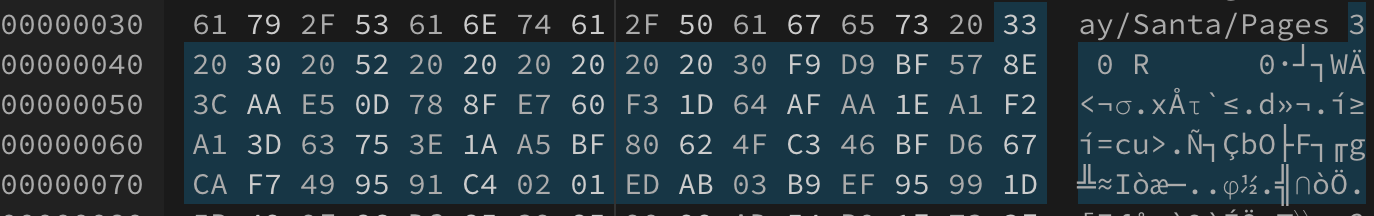
\includegraphics[scale=0.4]{pdf-change}
  \caption{Changed PDF.}
\end{figure}

By playing a bit (e.g. adding/subtracting with byte 33 -originally 32- ) we end up with a report mentioning that Jack Frost kicked a wombat. Since we added one byte there, we convert byte 1C to 1D and this wraps up the changes required in the PDF.

\subsection{Almost there}

Grinch knew what to do. He modified his code to load the PDF back and then dump the whole block.
Again, he modified his code a bit.
\begin{minted}{python}
with open('official_public.pem', 'rb') as fh:
        official_public_key = RSA.importKey(fh.read())
        c2 = Chain(load=True, filename='blockchain.dat')
        print('C2: Block chain verify: %s' % (c2.verify_chain(official_public_key, previous_hash='c6e2e6ecb785e7132c8003ab5aaba88d')))
        for block in c2.blocks:
            c2.save_a_block(block.index, filename='original.dat') # Save original block.
            h = SHA256.new()
            h.update(block.block_data_signed())
            if h.hexdigest() == '58a3b9335a6ceb0234c12d35a0564c4ef0e90152d0eb2ce2082383b38028a90f':
                hash  = block.full_hash()
                files = ['129459.bin', '129459.pdf']
                for i in range(2):
                    f = open('11b-collision/' + files[i], 'rb')
                    data = f.read()
                    block.data[i]['data'] = data
                block.sign = 0 # Drop him back to naughty.

                c2.save_a_block(block.index)
\end{minted}

By inspecting the two files, he identified where the Naughty/Nice status was. Also, he already knew that by converting him to Naughty, it means he subtracted, he had to add 1 to the 64th byte after that change.
The required change landed in the .bin file but he decided to load the whole block in a hex editor.

\begin{figure}[h!]
  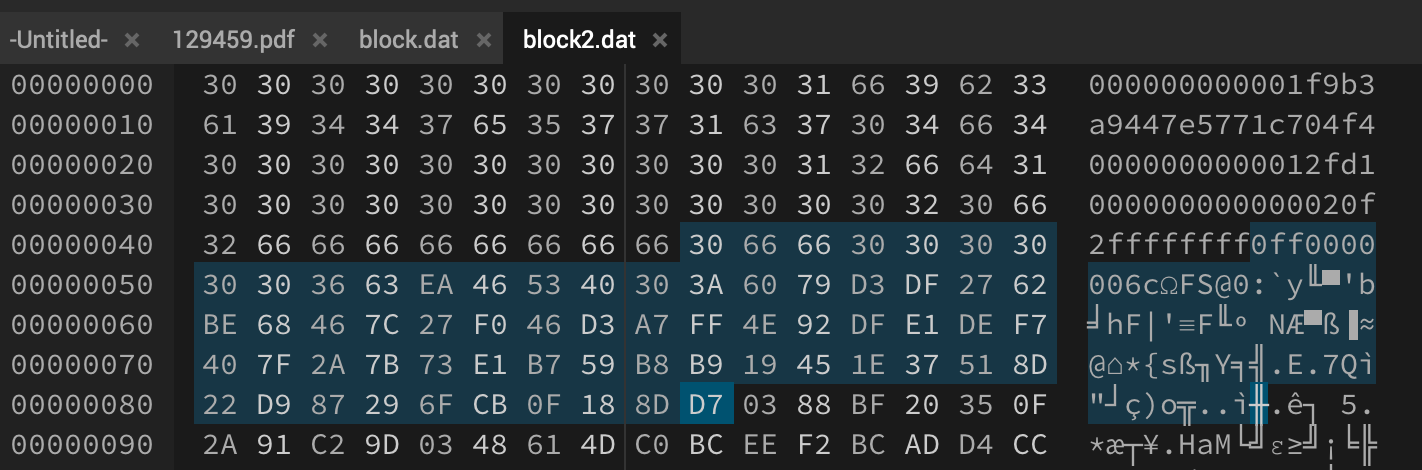
\includegraphics[scale=0.4]{last-change}
  \caption{Changed Block.}
\end{figure}

He changed byte with value 30 (originally 31), so he went ahead and +1 byte with D6 to D7.

Now, it was the time. Another quick modification of his script.
\begin{minted}{python}
if __name__ == '__main__':
    with open('official_public.pem', 'rb') as fh:
        official_public_key = RSA.importKey(fh.read())
        c2 = Chain(load=True, filename='blockchain.dat')
        print('C2: Block chain verify: %s' % (c2.verify_chain(official_public_key, previous_hash='c6e2e6ecb785e7132c8003ab5aaba88d')))
        for block in c2.blocks:
            h = SHA256.new()
            h.update(block.block_data_signed())
            if h.hexdigest() == '58a3b9335a6ceb0234c12d35a0564c4ef0e90152d0eb2ce2082383b38028a90f':
                hash  = block.full_hash()
                fh = open('block2.dat', 'rb')
                block2 = Block(load=True).load_a_block(fh)
                hash  = block.full_hash()
                hash2 = block2.full_hash()
                print (hash == hash2)
                h = SHA256.new()
                h.update(block2.block_data_signed())
                print(h.hexdigest())
\end{minted}

He ran the script and fff054f33c2134e0230efb29dad515064ac97aa8c68d33c58c01213a0d408afb.
He was quite happy, he saved christmas.
\subsection{Wait}
- Grinch, we are missing a narrative here.

- Oh, maybe I should stop pretending to be Santa and come back as myself and head to the balcony.
